\subsection{对称代数的函子性质}

命题 3. 设 A 为交换环，M 和 N 为两个 A-模，u: M → N 为 A-线性映射。则存在唯一的 A-代数同态 \(u'\) ：S(M) → S(N)，使得该图表

\pandocbounded{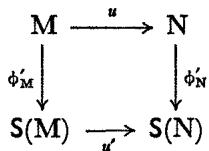
\includegraphics[keepaspectratio]{images/part003_0f38c769.jpg}}

是交换的。此外， \(u'\) 是分次代数同态。

\(u'\) 的存在性与唯一性由第 1 号命题 2 应用于交换代数 \(\mathbf{S}(\mathbf{N})\) 和 \(f = \phi_{\mathbf{N}}' \circ u: \mathbf{M} \to \mathbf{S}(\mathbf{N})\) 得出；由于

\[
f (\mathbf {M}) \subset \mathbf {S} ^ {1} (\mathbf {N}) = \mathbf {N},
\]

\(u'\) 是分次代数同态这一事实由第 1 号注记 1 得出。

命题 3 中的同态 \(u'\) 此后将记为 \(S(u)\) 。若 \(P\) 是一个 A-模，且 \(v: N \to P\) 是一个 A-线性映射，则

\[
\mathbf {S} (v \circ u) = \mathbf {S} (v) \circ \mathbf {S} (u)\tag{3}
\]

因为 \(\mathbf{S}(v) \circ \mathbf{S}(u)\) 是使下图交换的代数同态

\pandocbounded{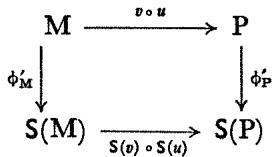
\includegraphics[keepaspectratio]{images/part003_67e6d402.jpg}}

由于 \(\mathbf{S}(\mathbf{M})\) 包含 \(\mathbf{M} = \mathbf{S}^1 (\mathbf{M})\) , \(\mathbf{S}(u)\) 有时称为 \(u\) 到 \(\mathbf{S}(\mathbf{M})\) 的典范扩张。限制 \(\mathbf{S}^n (u): \mathbf{S}^n (\mathbf{M}) \to \mathbf{S}^n (\mathbf{N})\) 满足

\[
\mathsf {S} ^ {n} (u) \left(x _ {1} x _ {2} \dots x _ {n}\right) = u \left(x _ {1}\right) u \left(x _ {2}\right) \dots u \left(x _ {n}\right)
\]

其中 \(x_{i} \in M\) ，因为 \(\mathbf{S}(u)\) 是一个代数同态且 \(\mathbf{S}^{1}(u) = u\) ；\(\mathbf{S}^{0}(u)\) 在 A 上的限制是恒等映射。注意， \(\mathbf{S}^{n}(u)\) 可以由 \(\mathbf{T}^{n}(u): \mathbf{T}^{n}(\mathbf{M}) \to \mathbf{T}^{n}(\mathbf{N})\) 通过过渡到商得到。

命题4. 若 \(u: \mathbf{M} \to \mathbf{N}\) 是满射 A-线性映射，则同态 \(\mathbf{S}(u): \mathbf{S}(\mathbf{M}) \to \mathbf{S}(\mathbf{N})\) 是满射的，且其核是 \(\mathbf{S}(\mathbf{M})\) 的由核 \(\mathbf{P} \subset \mathbf{M} \subset \mathbf{S}(\mathbf{M})\) （即 \(u\) 的核）生成的理想。

我们记 \(v = \mathsf{T}(u) \colon \mathsf{T}(\mathbf{M}) \to \mathsf{T}(\mathbf{N})\) ；我们知道（§5，第 2 号，命题 3） \(v\) 是满射的，因此由定义可知 \(v(\mathfrak{J}_{\mathbf{M}}') = \mathfrak{J}_{\mathbf{N}}'\) ；若 \(\Re\) 是 \(v\) 的核，则 \(v^{-1}(\mathfrak{J}_{\mathbf{N}}') = \Re + \mathfrak{J}_{\mathbf{M}}'\) 。由于 \(\mathsf{S}(u) \colon \mathsf{T}(\mathbf{M}) / \mathfrak{J}_{\mathbf{M}}' \to \mathsf{T}(\mathbf{N}) / \mathfrak{J}_{\mathbf{N}}'\) 是由 \(v\) 过渡到商而得到的，它是一个满射同态，其核为 \(\Re' = (\Re + \mathfrak{J}_{\mathbf{M}}') / \mathfrak{J}_{\mathbf{M}}'\) 。由于 \(\Re\) 由核 \(\mathbf{P}\) （即 \(u\) 的核）生成（§5，第 2 号），\(\Re'\) 亦然。

若 \(u: \mathbf{M} \to \mathbf{N}\) 是单射线性映射，\(\mathbf{S}(\mathbf{u})\) 并不总是单射映射（练习1）。然而，当 \(u\) 是使 \(u(\mathbf{M})\) 为 \(\mathbf{N}\) 中直因子的单射时，它是单射的，且此时 \(\mathbf{S}(u)\) 的像（同构于 \(\mathbf{S}(\mathbf{M})\) ）是 \(\mathbf{S}(\mathbf{N})\) 的一个直因子；其证明与关于 \(\mathbf{T}(u)\) 的类似断言（ \(\S 5\) ，第 2 号）的证明相同，只需把 \(\mathbf{T}\) 换为 \(\mathbf{S}\) 。

命题5. 设N和P是A-模M的两个子模，使得它们的和 \(N + P\) 是M中的直因子，且它们的交集 \(N \cap P\) 是N和P中的直因子。则同态 \(\mathsf{S}(\mathsf{N}) \to \mathsf{S}(\mathsf{M}), \mathsf{S}(\mathsf{P}) \to \mathsf{S}(\mathsf{M})\) 和

\[
\mathbf {S} (\mathbf {N} \cap \mathbf {P}) \rightarrow \mathbf {S} (\mathbf {M}),
\]

（即典范单射的典范扩张）都是单射的；如果 \(\mathbf{S}(\mathbf{N})\) , \(\mathbf{S}(\mathbf{P})\) 和 \(\mathbf{S}(\mathbf{N} \cap \mathbf{P})\) 通过这些同态被等同于 \(\mathbf{S}(\mathbf{M})\) 的子代数，则

\[
\mathbf {S} (\mathbf {N} \cap \mathbf {P}) = \mathbf {S} (\mathbf {N}) \cap \mathbf {S} (\mathbf {P}).\tag{4}
\]

证明归结为 §5，第 2 号，命题 4 的证明，只需通篇把 T 换为 S。当A是域时，命题5的假设对M的任意子模N、P总是成立。

推论。设K是一个交换域，M是K上的一个向量空间。对于每一个元素 \(z \in \mathbb{S}(\mathbf{M})\) 存在 M 的一个最小向量子空间 N，使得 \(z \in \mathbb{S}(\mathbf{N})\) 且N是有限维的。

证明的推导源自 §5，第 2 号，命题 4 的推论，只需通篇把 T 换为 S。

N 称为 M 的与 z 相关联的向量子空间。

